\section{Regions of interest}

The regions of interest (ROIs) were chosen as pixel locations in the image on specific places of the hand. ROI were selected on behalf of getting a full representation of the hand. 
Regions in the fingertips and nail folds are areas where it is easy to access the microcirculatory hemodynamics of the human body according to\cite{Iabichella2006}. 
%This region should therefore be expected to give some information on the changes in capillaries which can be an effect of vasomotion. 

The raw image on \figref{fig:hand} does not provide very good contrast for identifying ROIs. To easier choose ROIs, the raw image was converted to a gray scale image to improve the contrast in the image, this can be seen in \figref{fig:mat2grayHand}. 

\begin{figure}[H]
	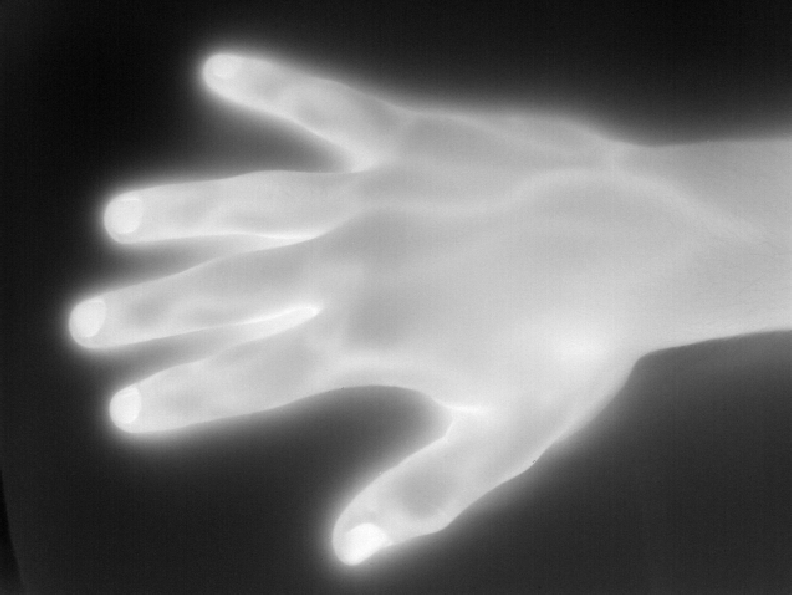
\includegraphics[width=0.6\textwidth]{figures/mat2grayHand}  %<--but is not needed.
	\caption{High contrast thermal image for subject 1.}
	\label{fig:mat2grayHand}  %<--give the figure a label, so you can reference!
\end{figure}

With the improved contrast, 28 ROIs from the hand were chosen on the first image of the thermal image series, by finding the coordinates of the pixels in the image. The regions are illustrated on \figref{fig:roiHand}. The localization of the regions is originating from the fingertips and elongating down the hand to the beginning of the wrist. Each region gives a pixel intensity value from one pixel of the image. In the setup of this study one pixel corresponds to an area on the hand with a diameter of about 417$\mu$m. Based on the fact, that the capillaries have an average diameter of 8$\mu$m\cite{martini2012}, it is sufficient to represent each region with just one pixel. Even the area represented by one pixel contains more than one capillary.

\begin{figure}[H]
	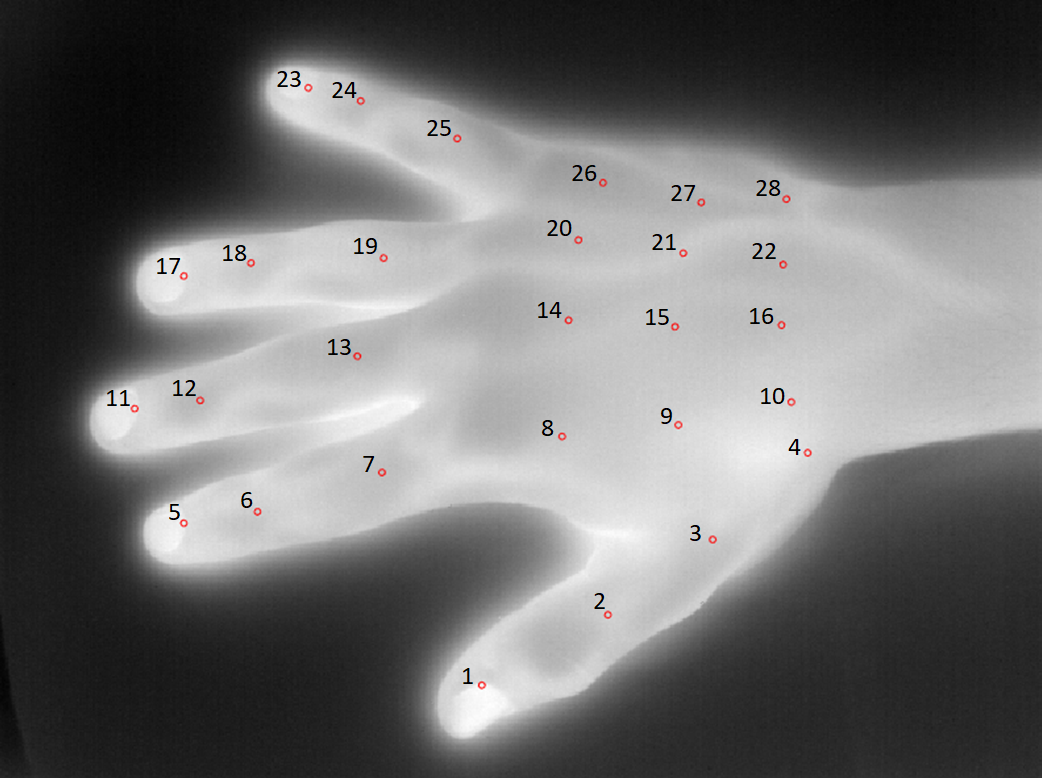
\includegraphics[width=0.6\textwidth]{figures/roiHand}  %<--but is not needed.
	\caption{First thermal image of subject 1's recording while restriction, with ROI of interest plottet on 28 areas of the hand represented as red circles.}
	\label{fig:roiHand}  %<--give the figure a label, so you can reference!
\end{figure}

The regions are fixed within the image matrix for the whole image series for each measurement, assuming that the subject was sitting still during the whole data acquisition period. The regions also account for both the baseline and restriction recording for each subject, assuming that the position of the hand was at the same position in both conditions. 
Iterating over the image series saving ROIs into a cell array with data points for each ROI, a vector for the each of the 28 ROI was made to give the pixel intensity variations over the whole measurement. 
An example of the pixel intensities for subject 1 is shown on \figref{fig:Intensities}.

\begin{figure}[H]
	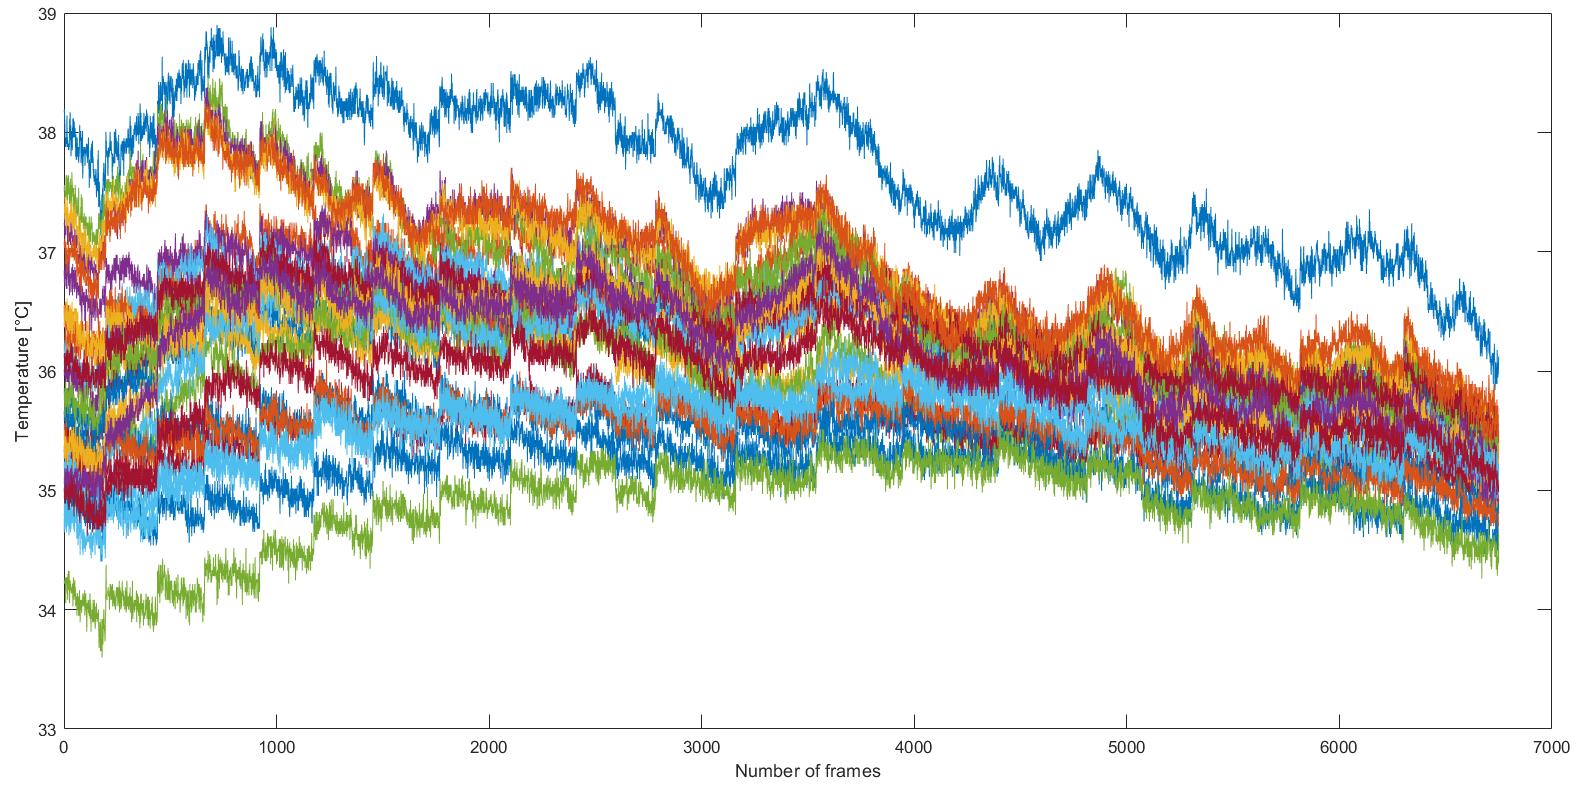
\includegraphics[width=1\textwidth]{figures/Intensities}  %<--but is not needed.
	\caption{Pixel intensity for all 28 ROIs during the restriction measurement of subject 1.}
	\label{fig:Intensities}  %<--give the figure a label, so you can reference!
\end{figure}

%It is noticed that there are some jumps at specific times in the pixel intensity for all ROI, this is due to the drift auto correction from the camera shutter \fixme{a citation of reference to another place should be here for documentation}. This problem is dealt with in the next section. %something like that...? dunno if it is to much to take the intensity plot with here? but i was thinking it to be to make a smooth transition to the drift correction... 